Welcome to the third assignment! During this assignment, you will practice your
math skills in an environment more similar to the one that you will face during
the course assessment. Although the questions will not be the same, they will
follow the same structure and you will have to solve the exercises using the
Dirac notation or matrix--vector multiplication.

Together with this assignment, you will find the \LaTeX { template} for you to
use when solving the exercises and writing down your answers. Remember to
upload a single pdf file with the full development of the assignment and the
answers.

\begin{question}
Are the quantum states $\ket{\psi_{1}} = \ket{00}$ and $\ket{\psi_{2}} = \ket{++}$ mutually orthogonal?
\label{qst:assignment3_1}
\end{question}
{\small
\texttt{Write down your solution here:}
\begin{equation*}
  \begin{split}
  \end{split}
\end{equation*}}
\vspace{0.1cm}

\begin{question}
Let $\ket{\psi} = \frac{4}{5} \ket{00} + \frac{2}{5} \ket{01} + \frac{2}{5} \ket{10} + \frac{1}{5} \ket{11}$. What is the probability of obtaining $M(q_{1} = 0)$ when measuring the system?
\label{qst:assignment3_2}
\end{question}
{\small
\texttt{Write down your solution here:}
\begin{equation*}
  \begin{split}
    \Prob{q_{1} = 0} &=  \\
  \end{split}
\end{equation*}}
\vspace{0.1cm}

\begin{question}
What is the resulting transformation matrix $T_{1}$ when applied the following operation $T_{1} = Y \otimes S$
\label{qst:assignment3_3}
\end{question}
{\small
\texttt{Write down your solution here:}
\begin{equation*}
  \begin{split}
    T_{1} &=  \\
  \end{split}
\end{equation*}}
\vspace{0.1cm}

\begin{figure}[t]
  \centerline{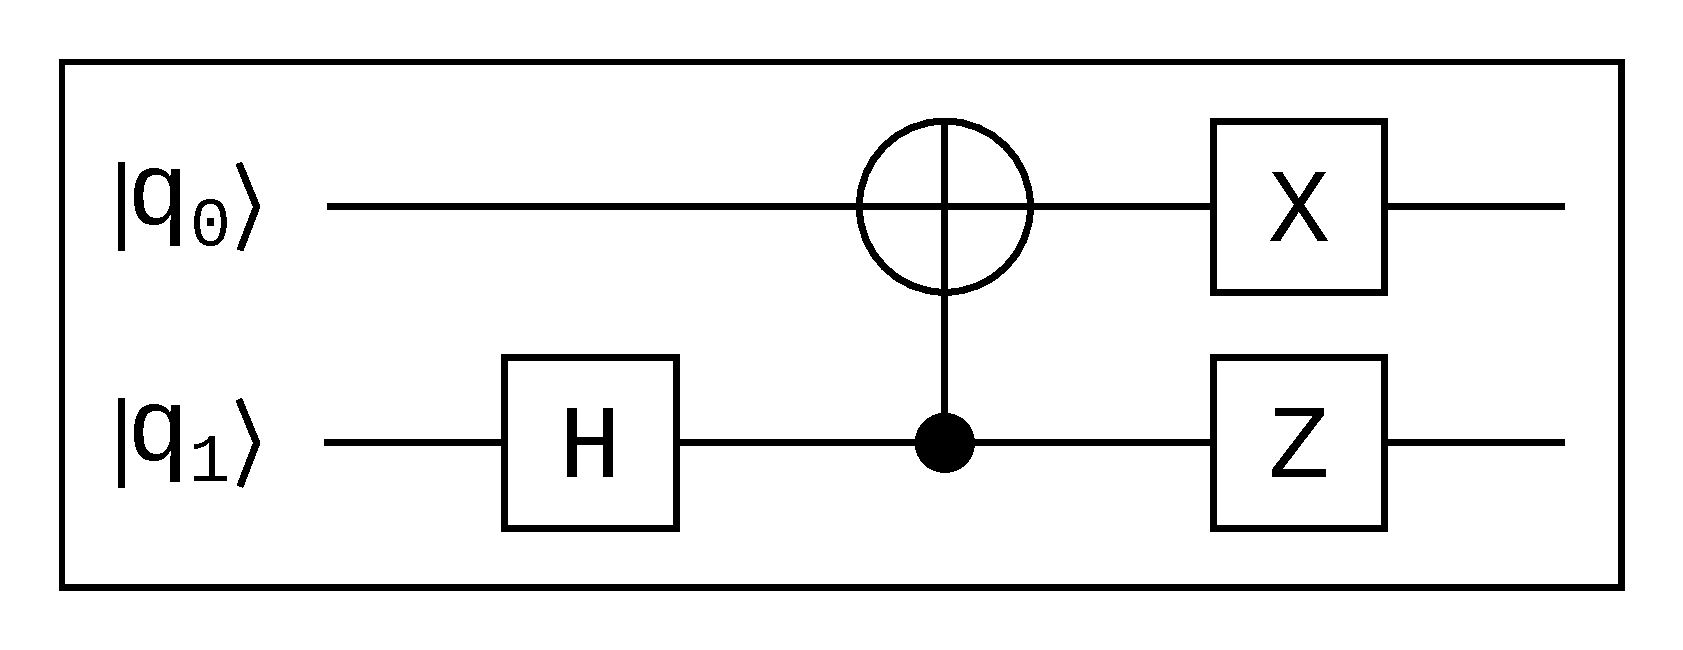
\includegraphics[scale=0.25]{img/qci_a3_question4.ps}}
  \caption{An arbitrary quantum circuit.}
  \label{fig:circuit2}
\end{figure}

\begin{question}
Consider the quantum circuit presented in Figure~\ref{fig:circuit2} and assume $\ket{q_{1}} = \ket{1}$ and $\ket{q_{0}} = \ket{0}$; hence, $\ket{\psi_{in}} = \ket{10}$. Determine, by using the matrix--vector multiplication, what is the state vector of the quantum circuit just before the measurement?
\label{qst:assignment3_4}
\end{question}
{\small
\texttt{Write down your solution here:}
\begin{equation*}
  \begin{split}
  \end{split}
\end{equation*}}
\vspace{0.1cm}

\begin{question}
Consider the quantum circuit presented in Figure~\ref{fig:circuit2} and assume $\ket{q_{1}} = \ket{0}$ and $\ket{q_{0}} = \ket{1}$; hence, $\ket{\psi_{in}} = \ket{01}$. Determine, by using the Dirac notation, what is the state vector of the quantum circuit just before the measurement?
\label{qst:assignment3_5}
\end{question}
{\small
\texttt{Write down your solution here:}
\begin{equation*}
  \begin{split}
      &\rightarrow \ket{01} \\
  \end{split}
\end{equation*}}
\vspace{0.1cm}

\begin{figure}[t]
  \centerline{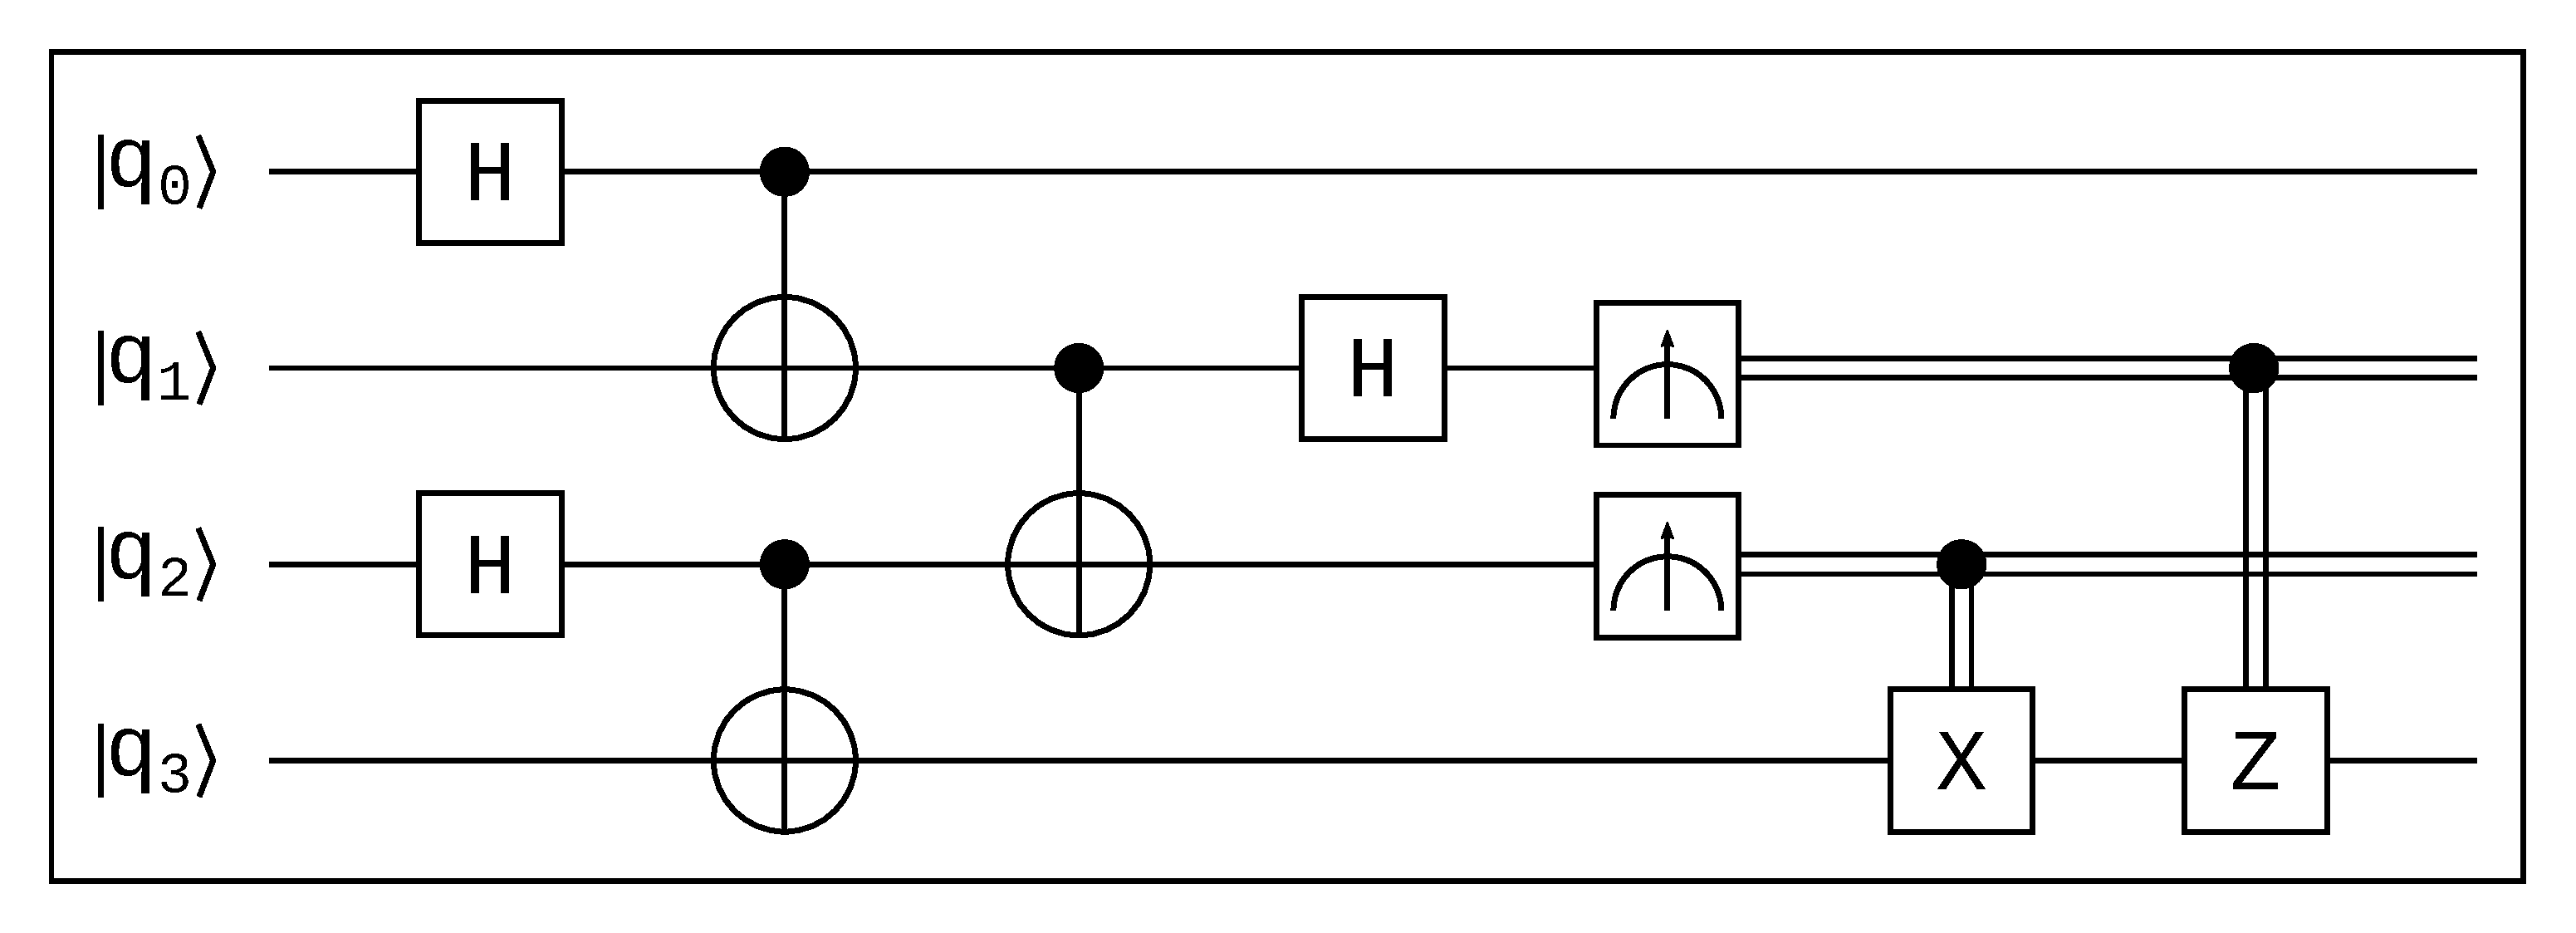
\includegraphics[scale=0.25]{img/qci_a3_question6.ps}}
  \caption{An arbitrary quantum circuit.}
  \label{fig:circuit3}
\end{figure}

\begin{question}
Consider the quantum circuit presented in Figure~\ref{fig:circuit3} and assume $\ket{q_{0}} = \ket{0}$, $\ket{q_{1}} = \ket{0}$, $\ket{q_{2}} = \ket{0}$ and $\ket{q_{3}} = \ket{0}$; hence, $\ket{\psi_{in}} = \ket{0000}$. Determine, by using the Dirac notation, what is the state vector of the quantum circuit just before the partial measurement?
\label{qst:assignment3_6}
\end{question}
{\small
\texttt{Write down your solution here:}
\begin{equation*}
  \begin{split}
    &\rightarrow \ket{0000} \\
  \end{split}
\end{equation*}}
\vspace{0.1cm}

\begin{question}
Considering the state vector obtained in Question~\ref{qst:assignment3_6}. What is the probability  $\Prob{q_{3} = 1}$?
\label{qst:assignment3_7}
\end{question}
{\small
\texttt{Write down your solution here:}
\begin{equation*}
  \begin{split}
    \Prob{q_{3} = 1} &=  \\
  \end{split}
\end{equation*}}
\vspace{0.1cm}

\begin{question}
Considering the state vector obtained in Question~\ref{qst:assignment3_6}. Assume that the measuring process returned the following values: $M(\ket{q_{2}}) = 1$ and $M(\ket{q_{1}}) = 0$. What is the state vector of the quantum circuit after the described partial measurement? (Note: Remember to renormalize the vector).
\label{qst:assignment3_8}
\end{question}
{\small
\texttt{Write down your solution here:}
\begin{equation*}
  \begin{split}
  \end{split}
\end{equation*}}
\vspace{0.1cm}

\begin{question}
Considering the state vector and the measurements indicated in Question~\ref{qst:assignment3_8}. What is the final state vector of the quantum circuit after applying the corrections?
\label{qst:assignment3_9}
\end{question}
{\small
\texttt{Write down your solution here:}
\begin{equation*}
  \begin{split}
  \end{split}
\end{equation*}}
\vspace{0.1cm}

\begin{question}
Considering the state vector obtained in Question~\ref{qst:assignment3_6}. Assume that the measuring process returned the following values: $M(\ket{q_{2}}) = 1$ and $M(\ket{q_{1}}) = 1$. What is the final state vector of the quantum circuit after applying the corrections? (Note: Remember to renormalize the vector).
\label{qst:assignment3_10}
\end{question}
{\small
\texttt{Write down your solution here:}
\begin{equation*}
  \begin{split}
  \end{split}
\end{equation*}}
